\documentclass{standalone}
\usepackage[utf8x]{inputenc}
\usepackage[T1]{fontenc}
\usepackage{libertine}
\usepackage[usenames,dvipsnames,x11names,table,svgnames]{xcolor}
\usepackage{tikz}
\usetikzlibrary{mindmap,trees,backgrounds,calc}

\begin{document}
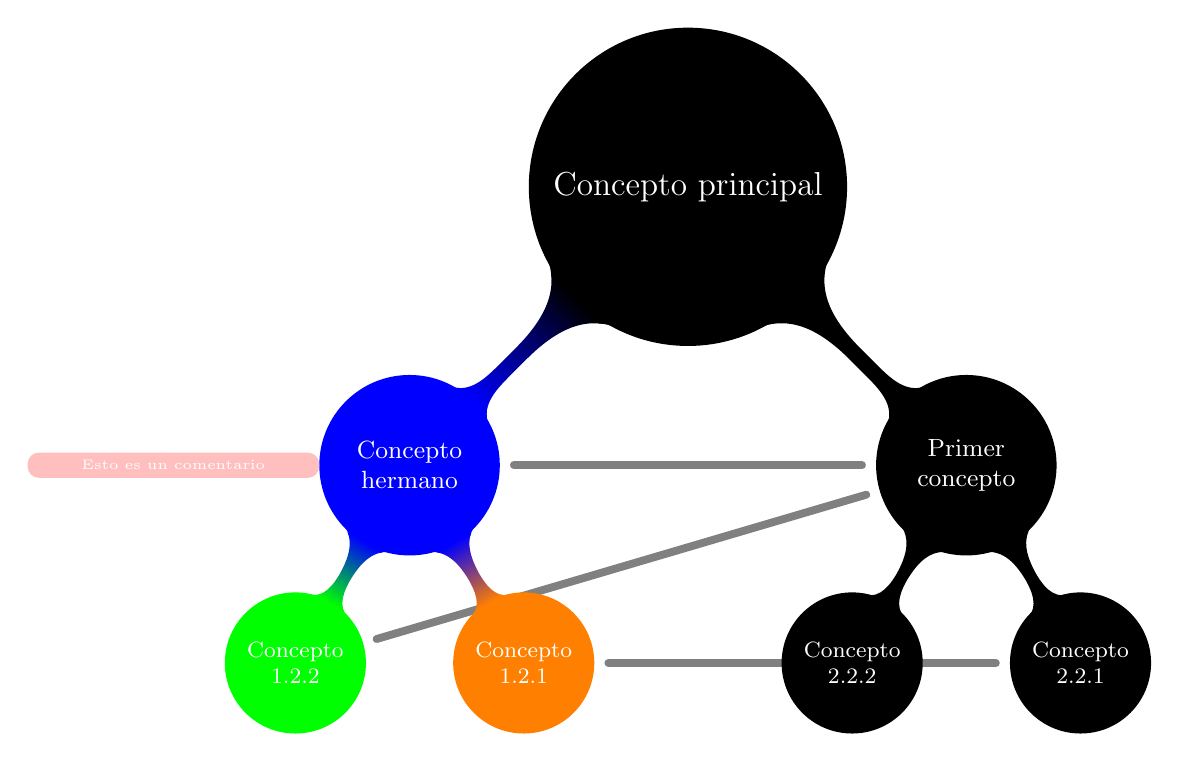
\begin{tikzpicture}[mindmap, concept color = black,
text = white, every annotation/.style = {fill = red!25}]

\tikzset{
	root_concept/.append style = {
		concept color = black
	},
	level1_concept/.append style = {
		concept color = blue
	},
	level2_concept/.append style = {
		concept color = green!75!black
	}
}

\node[concept] {Concepto principal} % Concepto Raíz
	child[grow = -45] { %, concept color = blue
		node[concept] (PC) {Primer concepto} [clockwise from = -60]
			child{node[concept] (C221) {Concepto 2.2.1}}
			child{node[concept] (C222) {Concepto 2.2.2}}
	} %Nivel 1
	child[grow = 225, concept color = blue] { %concept color = green!75!black
		node[concept] (CH) {Concepto hermano} [clockwise from = -60]		child[concept color = orange]{node[concept] (C121) {Concepto 1.2.1}}
		%,concept color = orange
		child[concept color = green!]{node[concept] (C122) {Concepto 1.2.2}}
	}; % Nivel 1 child ``hace crecer''
\node[annotation, left, align = center] at ($(CH)+ (-1,0)$) {Esto es un comentario};
%CH.east
\begin{pgfonlayer}{background}
\draw[concept connection] (PC) edge (CH); % De mindmap, ¿qué significa edge?
\draw[concept connection] (C121) edge (C221);
\draw[concept connection] (PC) edge (C122);
\end{pgfonlayer}
\end{tikzpicture}
\end{document}